% !TEX root = ../../ozan_sener_thesis.tex
\begin{figure}
\centering
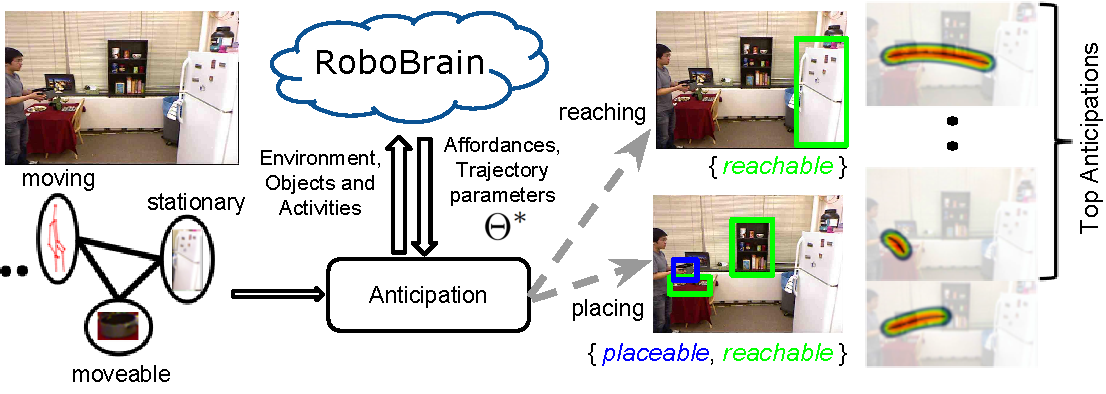
\includegraphics[width=\linewidth]{./Image/anticipation_robobrain_pic.pdf}
\caption{\textbf{\robobrain{} for anticipating human activities.} Robot using anticipation algorithm of \citet{KoppulaRSS2013} queries \robobrain{}, for the activity, affordance and trajectory parameters in order to generate and rank the possible future activities in a given environment.}
\label{Fig:anticipation}
\end{figure}

\subsubsection{Anticipating human actions}
\label{sec:anticipation}
The assistive robots working with humans should be able to understand human activities and also anticipate the future actions that the human can perform. In order to anticipate, the robot should reason over the action possibilities in the environment, i.e., \textit{object affordances}, and how the actions can be performed, i.e., \textit{trajectories}. Several works in robotics have addressed the problem of anticipation~\citep{KitaniECCV2012,KoppulaRSS2013,Kuderer-RSS-12}.

We now show how robots can query \robobrain{} and use the previous work by
Koppula et al.~\citep{KoppulaRSS2013} for anticipating human actions.  
In order to anticipate the future human actions, the authors~\citep{KoppulaRSS2013} learn parameters using their anticipatory algorithm, and using the learned parameters they anticipate the most likely \textit{future} object affordances and human trajectories. \robobrain{} serves anticipation \textit{as-a-service} by storing those learned parameters, object affordances and trajectories  as concepts in its graph. Figure~\ref{Fig:anticipation} illustrates a robot retrieving relevant information for anticipation. The robot first uses the following queries to retrieve the possible trajectories of an object:

%\noindent \resizebox{\linewidth}{!}{
%\begin{minipage}{\linewidth}
{\small
\begin{align}
&{\tt {affordances} \,\, n := fetch \,\,(\{name:n\})\rightarrow   [`HasAffordance'] \rightarrow } \cr
& {\tt \hspace*{2cm} (v\{src:`Affordance'\})   \nonumber } \\
&{\tt {trajectories} \,\, a := fetch \,\,(\{handle:a\})\rightarrow [`HasParameters']\rightarrow } \cr
& {\tt \hspace*{2cm}  (v\{src:`Affordance', type:`Trajectory'\})  \nonumber } \\
& {\tt { trajectory\_parameters} \,\, o := \,\, } \cr
&{\tt \hspace*{2cm} map (\lambda a \rightarrow {trajectories}\,\, a)  \,\, {affordances}\,\, o } \nonumber
\end{align}
%  \end{minipage}
}


In the queries above, the robot first queries for the affordances of the object and then for each affordance it queries \robobrain{} for the trajectory parameters. Having retrieved all possible trajectories, the robot uses the learned parameters~\citep{KoppulaRSS2013} to anticipate the future human actions. Since the learned parameters are also stored in the \robobrain{} graph, the robot retrieves them using the following RQL queries:
{\small
\begin{align*}
&{\tt {parents} \,\, n := fetch \,\, (v)\rightarrow [`HasParameters']\rightarrow  (\{handle:n\}) }\nonumber \\
& {\tt {parameters} \,\, n :=  fetch \,\, (\{name:n\})\rightarrow [`HasParameters']\rightarrow }\cr
& {\tt \hspace*{2cm}  (v\{src:`Activity'\})   \nonumber } \\
& {\tt find\_parameters\, a := }\\
& \hspace*{2cm}{\tt filter (\lambda u \rightarrow\! {Len\; parents}\, u = 1)     {parameters}\, a \nonumber } \\
& {\tt {joint\_parameters} \,\, a_1 \,\, a_2\,\, := filter (\lambda u \rightarrow {Len\; parents}\,\, u = 2\,\, } \cr
& {\tt \hspace*{2cm}  and\,\, u \,\, in \,\, {parameters}\,\, a_2)    \,\,{parameters}\,\, a_1 \nonumber}
\end{align*}
}
The queries above retrieves both independent and joint parameters for anticipating the object affordances and human activities. Detailed explanation of the query is given in Example \ref{ex:joint} of Section \ref{sec:raquel}


